% Allowed document classes: cls/Bohr_Sci, cls/Sci, cls/SAI
\documentclass[11pt, a4paper, logo, copyright, nonumbering]{cls/Sci}
\usepackage[authoryear, sort&compress, round]{natbib}
\usepackage{dblfloatfix}
\usepackage{ulem}
\usepackage{caption}
\captionsetup{
  justification=justified,
  singlelinecheck=false
}
\usepackage{dramatist}
\usepackage{xspace}
\usepackage{pifont} %
\usepackage{multirow}
\usepackage{tcolorbox}
\usepackage{xltabular}
\usepackage{longtable}
\usepackage{hyperref}
\interfootnotelinepenalty=10000

\usepackage{amsfonts}
\usepackage{amsmath}
\usepackage{amssymb}
\usepackage{lineno}
\usepackage{multirow}
\usepackage{adjustbox}

\usepackage[bottom]{footmisc}

\usepackage{CJKutf8}
\usepackage{subfigure}
\usepackage{setspace}

\usepackage{dsfont}
\usepackage{array} %
\usepackage{tabularx} %
\usepackage{subfigure} %
\usepackage{xcolor} %
\usepackage{tabularx}
\usepackage{booktabs}

\usepackage{lipsum}  %
\usepackage{multicol} %

\usepackage{booktabs}
\usepackage{multirow}  
\usepackage{color} 
\usepackage[table]{xcolor}

\usepackage{placeins}


\makeatletter
\def\@BTrule[#1]{%
  \ifx\longtable\undefined
    \let\@BTswitch\@BTnormal
  \else\ifx\hline\LT@hline
    \nobreak
    \let\@BTswitch\@BLTrule
  \else
     \let\@BTswitch\@BTnormal
  \fi\fi
  \global\@thisrulewidth=#1\relax
  \ifnum\@thisruleclass=\tw@\vskip\@aboverulesep\else
  \ifnum\@lastruleclass=\z@\vskip\@aboverulesep\else
  \ifnum\@lastruleclass=\@ne\vskip\doublerulesep\fi\fi\fi
  \@BTswitch}
\makeatother

\addto\extrasenglish{
    \def\chapterautorefname{Chapter}%
    \def\sectionautorefname{Section}%
    \def\paragraphautorefname{Section}
    \def\subparagraphautorefname{Section}
    \def\paragraphautorefname{Paragraph}%
    \def\tableautorefname{Table}%
    \def\equationautorefname{Equation}%
}

\newenvironment{indentchunk}[1]%
 {\begin{list}{}%
         {\setlength{\leftmargin}{#1}}%
         \item[]%
 }
 {\end{list}}

\bibliographystyle{abbrvnat}

\reportnumber{001} %


\title{EvoMaster: A Foundational Evolving Agent Framework for Agentic Science at Scale}

\author{
    Xinyu Zhu\textsuperscript{\rm 1,2, $\dagger$},
    Yuzhu Cai\textsuperscript{\rm 1,2, $\dagger$},
    Zexi Liu\textsuperscript{\rm 1,2, $\dagger$},
    
    Cheng Wang\textsuperscript{\rm 1},
    Fengyang Li\textsuperscript{\rm 1},
    Wenkai Jin\textsuperscript{\rm 1},
    Wanxu Liu\textsuperscript{\rm 1},
    Zehao Bing\textsuperscript{\rm 1},
    Bingyang Zheng\textsuperscript{\rm 1},
    
    Jingyi Chai\textsuperscript{\rm 1,2},
    Shuo Tang\textsuperscript{\rm 1,2},
    Rui Ye\textsuperscript{\rm 1},
    Yuwen Du\textsuperscript{\rm 1,2},
    Xianghe Pang\textsuperscript{\rm 1,2},
    Yaxin Du\textsuperscript{\rm 1},
    Tingjia Miao\textsuperscript{\rm 1},

    Yuzhi Zhang\textsuperscript{\rm 2},
    Ruoxue Liao\textsuperscript{\rm 3},
    Zhaohan Ding\textsuperscript{\rm 3},
    Linfeng Zhang\textsuperscript{\rm 3},
    Yanfeng Wang\textsuperscript{\rm 1},
    Weinan E\textsuperscript{\rm 1},
    Siheng Chen\textsuperscript{\rm 1, 2,$\ast$}
    \\
    \textsuperscript{\rm 1} School of Artificial Intelligence, Shanghai Jiao Tong University \\
    \textsuperscript{\rm 2} SciLand \quad  \textsuperscript{\rm 3} DP Technology 
}

\newcommand{\xmark}{\textcolor{red}{\ensuremath{\times}}}
\newcommand{\cmark}{\textcolor[rgb]{0,0.51,0}{\checkmark}}

\definecolor{lightgreen}{HTML}{E6F4EA}
\begin{document}

\begingroup
    \renewcommand{\thefootnote}{\fnsymbol{footnote}} 
    
    \footnotetext[2]{Equal contribution, alphabetical order by first name.} 
    

    \footnotetext[1]{Corresponding author: \texttt{sihengc@sjtu.edu.cn}}

\endgroup
\begin{abstract}
The convergence of large language models and agents is catalyzing a new era of scientific discovery: \textbf{Agentic Science}. While the scientific method is inherently iterative, existing agent frameworks are predominantly static, narrowly scoped, and lack the capacity to learn from trial and error. To bridge this gap, we present \textbf{EvoMaster}, a \textbf{foundational} evolving agent framework engineered specifically for \textbf{Agentic Science at Scale}. 
Driven by the core principle of \textbf{continuous self-evolution}, EvoMaster empowers agents to iteratively refine hypotheses, self-critique, and progressively accumulate knowledge across experimental cycles, faithfully mirroring human scientific inquiry. Crucially, as a domain-agnostic base harness, EvoMaster is exceptionally \textbf{easy to scale up}---enabling developers to build and deploy highly capable, self-evolving scientific agents for arbitrary disciplines in approximately 100 lines of code. 
Built upon EvoMaster, we incubated the SciMaster ecosystem across domains such as machine learning, physics, and general science. Evaluations on four authoritative benchmarks (Humanity's Last Exam, MLE-Bench Lite, BrowseComp, and FrontierScience) demonstrate that EvoMaster achieves state-of-the-art scores of 41.1\%, 75.8\%, 73.3\%, and 53.3\%, respectively. It comprehensively outperforms the general-purpose baseline OpenClaw with relative improvements ranging from +159\% to +316\%, robustly validating its efficacy and generality as the premier foundational framework for the next generation of autonomous scientific discovery. 

\medskip
\noindent
\includegraphics[width=1em]{figures/github.png}\quad\textbf{Code}\quad\href{https://github.com/sjtu-sai-agents/EvoMaster}{https://github.com/sjtu-sai-agents/EvoMaster}
\end{abstract}



\maketitle

\begin{figure}[t]
    \centering
    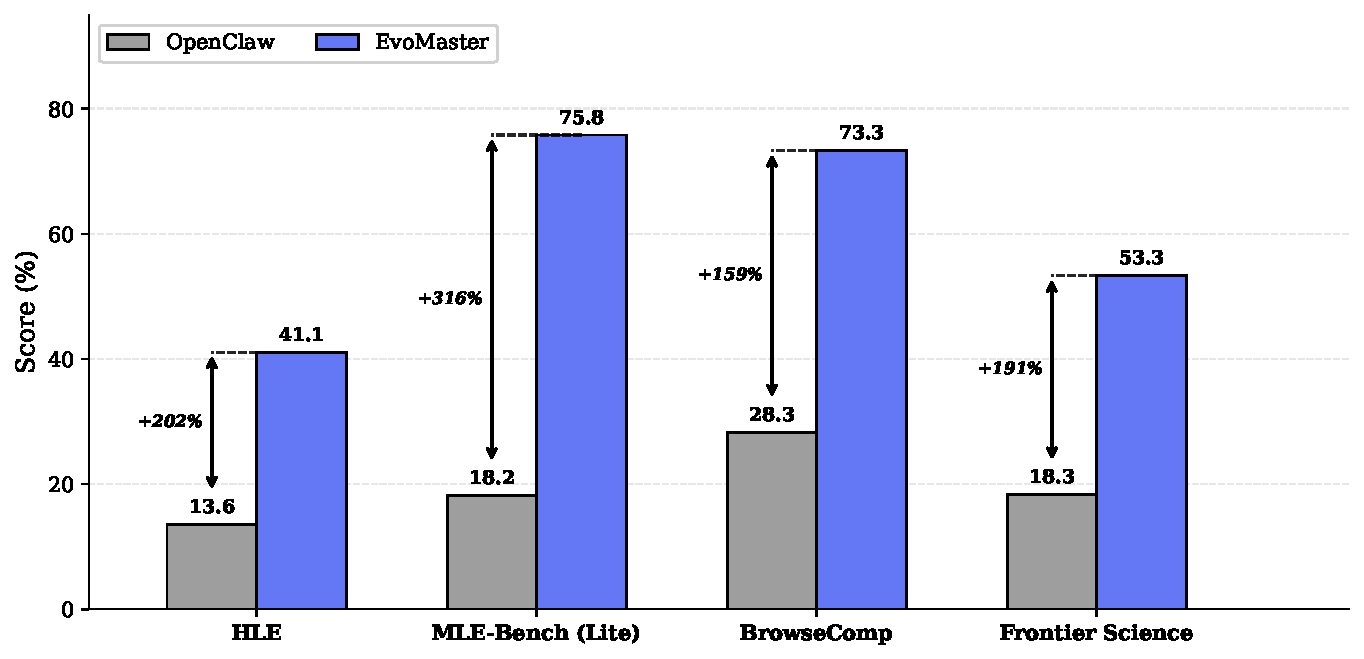
\includegraphics[width=0.92\textwidth]{figures/evomaster_vs_openclaw.pdf}
    \caption{Performance comparison between EvoMaster and OpenClaw across four authoritative benchmarks. EvoMaster consistently and substantially outperforms the general-purpose baseline, with relative improvements ranging from +159\% (BrowseComp) to +316\% (MLE-Bench Lite). Both methods use GPT-5.4 as the backend model.}
    \label{fig:teaser}
\end{figure}

%=====================================================================
\newpage
\section{Introduction}
\label{sec:intro}
%=====================================================================

\subsection{The Dawn of Agentic Science}

Large language models with strong reasoning, planning, and tool-use capabilities~\citep{openai2025agents, anthropic2025claude} are transforming the landscape of scientific research. A growing community consensus recognizes that AI agents represent the next frontier for accelerating scientific discovery~\citep{gottwaldtglobalcollaboration}. The 2024 Nobel Prizes in Physics and Chemistry, awarded to pioneers of artificial neural networks and computational protein design~\citep{nobelphysics2024, nobelchemistry2024}, signal that AI has moved to the center of scientific achievement. AlphaFold~\citep{jumper2021highly} and AlphaFold~3~\citep{abramson2024alphafold3} have revolutionized structural biology; GNoME~\citep{merchant2023scaling} discovered 2.2 million new crystal structures in a single sweep, equivalent to 800 years of human experimental work. Yet these achievements still position AI as a \emph{tool} that answers specific questions posed by human researchers. The emergence of autonomous agents that can independently drive the full cycle of scientific research, from literature review and hypothesis generation, through experimental design and code execution, to result analysis and paper writing, marks the arrival of \emph{\textbf{Agentic Science}}. Early demonstrations such as Coscientist~\citep{boiko2023autonomous} and The AI Scientist~\citep{lu2024aiscientist} confirm that this paradigm is imminently feasible.

If a single AI agent can conduct a complete research cycle in hours rather than months, the next imperative is to deploy such agents across dozens of scientific disciplines simultaneously. Scaling up not only extends coverage to more domains but also enables parallel execution that further accelerates discovery. We call this prospect \emph{\textbf{Agentic Science at Scale}}: the pace of scientific discovery is no longer bottlenecked by human bandwidth but by the quality of our AI agent architectures. This paper takes a foundational step toward that vision.

\subsection{Challenges of Agentic Science at Scale}

Despite its transformative promise, scaling Agentic Science from isolated demonstrations to a broadly applicable paradigm faces two critical challenges:



\textbf{Fragmented, siloed development.} Scientific research spans diverse disciplines. From chemistry and biology to materials science, each characterizes unique toolchains, data modalities, and evaluation protocols. Currently, most scientific agents are developed as monolithic, domain-specific systems: ChemCrow~\citep{bran2024augmenting} is custom-tailored for chemical synthesis, while systems like MLAgentBench~\citep{huang2023mlagentbench} are strictly coupled to machine learning pipelines. Such "bottom-up" engineering leads to a massive duplication of effort in common harness such as tool orchestration, trajectory management, and error recovery. This lack of a \textbf{foundational} abstraction layer ensures that advances in one domain remain non-transferable to others. Consequently, the marginal cost of supporting a new discipline remains prohibitively high, preventing the horizontal scaling of agentic capabilities across the broader scientific landscape.

\textbf{Absence of evolution.} Scientific discovery is inherently a long-horizon, trial-and-error process that aligns with the cycle of hypothesis, experimentation, and refinement. However, existing agent frameworks predominantly follow a single-pass paradigm: they execute a task once and terminate, lacking the mechanism to learn from failures or accumulate insights over successive attempts. This "stateless" execution contradicts the essence of the scientific method, where understanding is deepened through repeated iterations. Without the capacity for \textbf{continuous evolution}, agents remain static tools rather than self-improving researchers. They struggle to navigate complex, open-ended scientific frontiers that require the agent to progressively refine its strategies and "evolve" its cognitive boundaries through experimental feedback.

\subsection{EvoMaster: A Foundational Evolving Agent Framework for Agentic Science at Scale}
To address these challenges, we propose \textbf{EvoMaster}, a foundational evolving agent framework engineered specifically for \emph{Agentic Science at Scale}. EvoMaster is driven by two core tenets: serving as a \textbf{foundational} harness that unifies agent development across diverse disciplines, and driving \textbf{continuous evolution}, allowing agents to iteratively refine strategies and accumulate experience just as human researchers do. EvoMaster translates them directly into four architectural design principles:

\begin{itemize}[leftmargin=*, nosep]
    \item \textbf{Modular composability}: To provide a truly foundational platform, the system is decoupled into independently replaceable components managed by unified registries. This standardizes harness, enabling the seamless onboarding of new scientific domains with minimal marginal cost and fostering organic ecosystem growth.
    \item \textbf{Experiment-ready harness}: Agent behavior is governed by declarative configurations paired with comprehensive trajectory tracking. This guarantees the parameter agility and execution traceability essential for rigorous, cross-domain scientific experimentation.
    \item \textbf{Iterative self-evolution}: Breaking away from single-pass execution, EvoMaster agents operate within multi-turn reactive loops. Equipped with intelligent context management, agents continuously observe, self-critique, and refine their hypotheses over long horizons, faithfully mirroring the iterative scientific method.
    \item \textbf{Multi-agent collaborative evolution}: The orchestration layer supports flexible collaboration patterns, enabling agent teams to collectively debate and optimize solutions, simulating the peer-driven dynamics of real-world scientific discovery.
\end{itemize}

Built upon these principles and EvoMaster, we have successfully incubated the \textbf{SciMaster}~\citep{zhang2025bohrium+} agent ecosystem, which spans autonomous machine learning (ML-Master~2.0)~\citep{sjtu2025mlmaster, sjtu2026mlmaster2}, general scientific research (X-Master / X-Master 2.0)~\citep{sjtu2025xmaster}, web information retrieval (Browse-Master)~\citep{sjtu2025browsemaster}, physics reasoning (PhysMaster)~\citep{sjtu2025physmaster}, and embodied intelligence training (EmboMaster)~\citep{sjtu2026embomaster}. By leveraging a shared foundational harness, we are rapidly expanding this ecosystem to additional scientific domains.

To comprehensively validate the scientific and evolutionary capabilities of EvoMaster, we conduct head-to-head comparisons against OpenClaw~\citep{steinberger2025openclaw}, the fastest-growing open-source general AI agent. Rather than merely evaluating general intelligence, we deliberately selected four authoritative benchmarks that map directly to the core competencies required for Agentic Science:

\begin{itemize}[leftmargin=*, nosep]
\item \textbf{BrowseComp} evaluates deep, multi-step information retrieval. Since comprehensive literature review and data sourcing are the bedrock of research, EvoMaster's superior performance (73.3\%, \textbf{+159\%} relative gain) demonstrates its ability to autonomously navigate the web to extract and synthesize high-quality scientific context.
\item \textbf{MLE-Bench Lite} tests long-horizon machine learning engineering. Scientific discovery is inherently a prolonged, trial-and-error process. EvoMaster's state-of-the-art 75.8\% medal rate (\textbf{+316\%}) proves its structural capacity to sustain complex, multi-step experimental workflows over extended horizons without compounding errors.
\item \textbf{HLE} assesses cross-disciplinary expert knowledge. Modern breakthroughs often occur at the intersection of fields; achieving 41.1\% accuracy (\textbf{+202\%}) confirms EvoMaster possesses the robust, multidisciplinary cognitive foundation necessary for cross-domain hypothesis generation.
\item \textbf{FrontierScience} directly measures advanced reasoning across physics, chemistry, and biology. EvoMaster's strong performance (53.3\%, \textbf{+191\%}) serves as direct evidence that it can successfully resolve domain-specific, PhD-level scientific problems.
\end{itemize}

Specifically, as illustrated in Figure~\ref{fig:mlebench_time_medal}, EvoMaster demonstrates continuous self-evolution on the long-horizon MLE-Bench, progressively reaching superior accuracy. Together, these results systematically confirm that a domain-aware, evolution-driven framework comprehensively outperforms general-purpose platforms, effectively bridging the gap between isolated tools and fully autonomous scientific discovery.


% To validate the scientific and evolutionary capabilities of EvoMaster, we conduct head-to-head comparisons against OpenClaw~\citep{steinberger2025openclaw}, the fastest-growing open-source general AI agent, across four authoritative benchmarks. EvoMaster consistently achieves state-of-the-art performance: 41.1\% on HLE (vs.\ 13.6\%, \textbf{+202\%}), 75.8\% on MLE-Bench Lite (vs.\ 18.2\%, \textbf{+316\%}), 73.3\% on BrowseComp (vs.\ 28.3\%, \textbf{+159\%}), and 53.3\% on FrontierScience (vs.\ 18.3\%, \textbf{+191\%}). Specifically, as illustrated in Figure~\ref{fig:mlebench_time_medal}, EvoMaster demonstrates continuous self-evolution on the long-horizon MLE-Bench, progressively reaching superior accuracy. These results systematically confirm that a domain-aware, evolution-driven framework comprehensively outperforms general-purpose platforms in rigorous scientific tasks.

\begin{figure}[t]
    \centering
    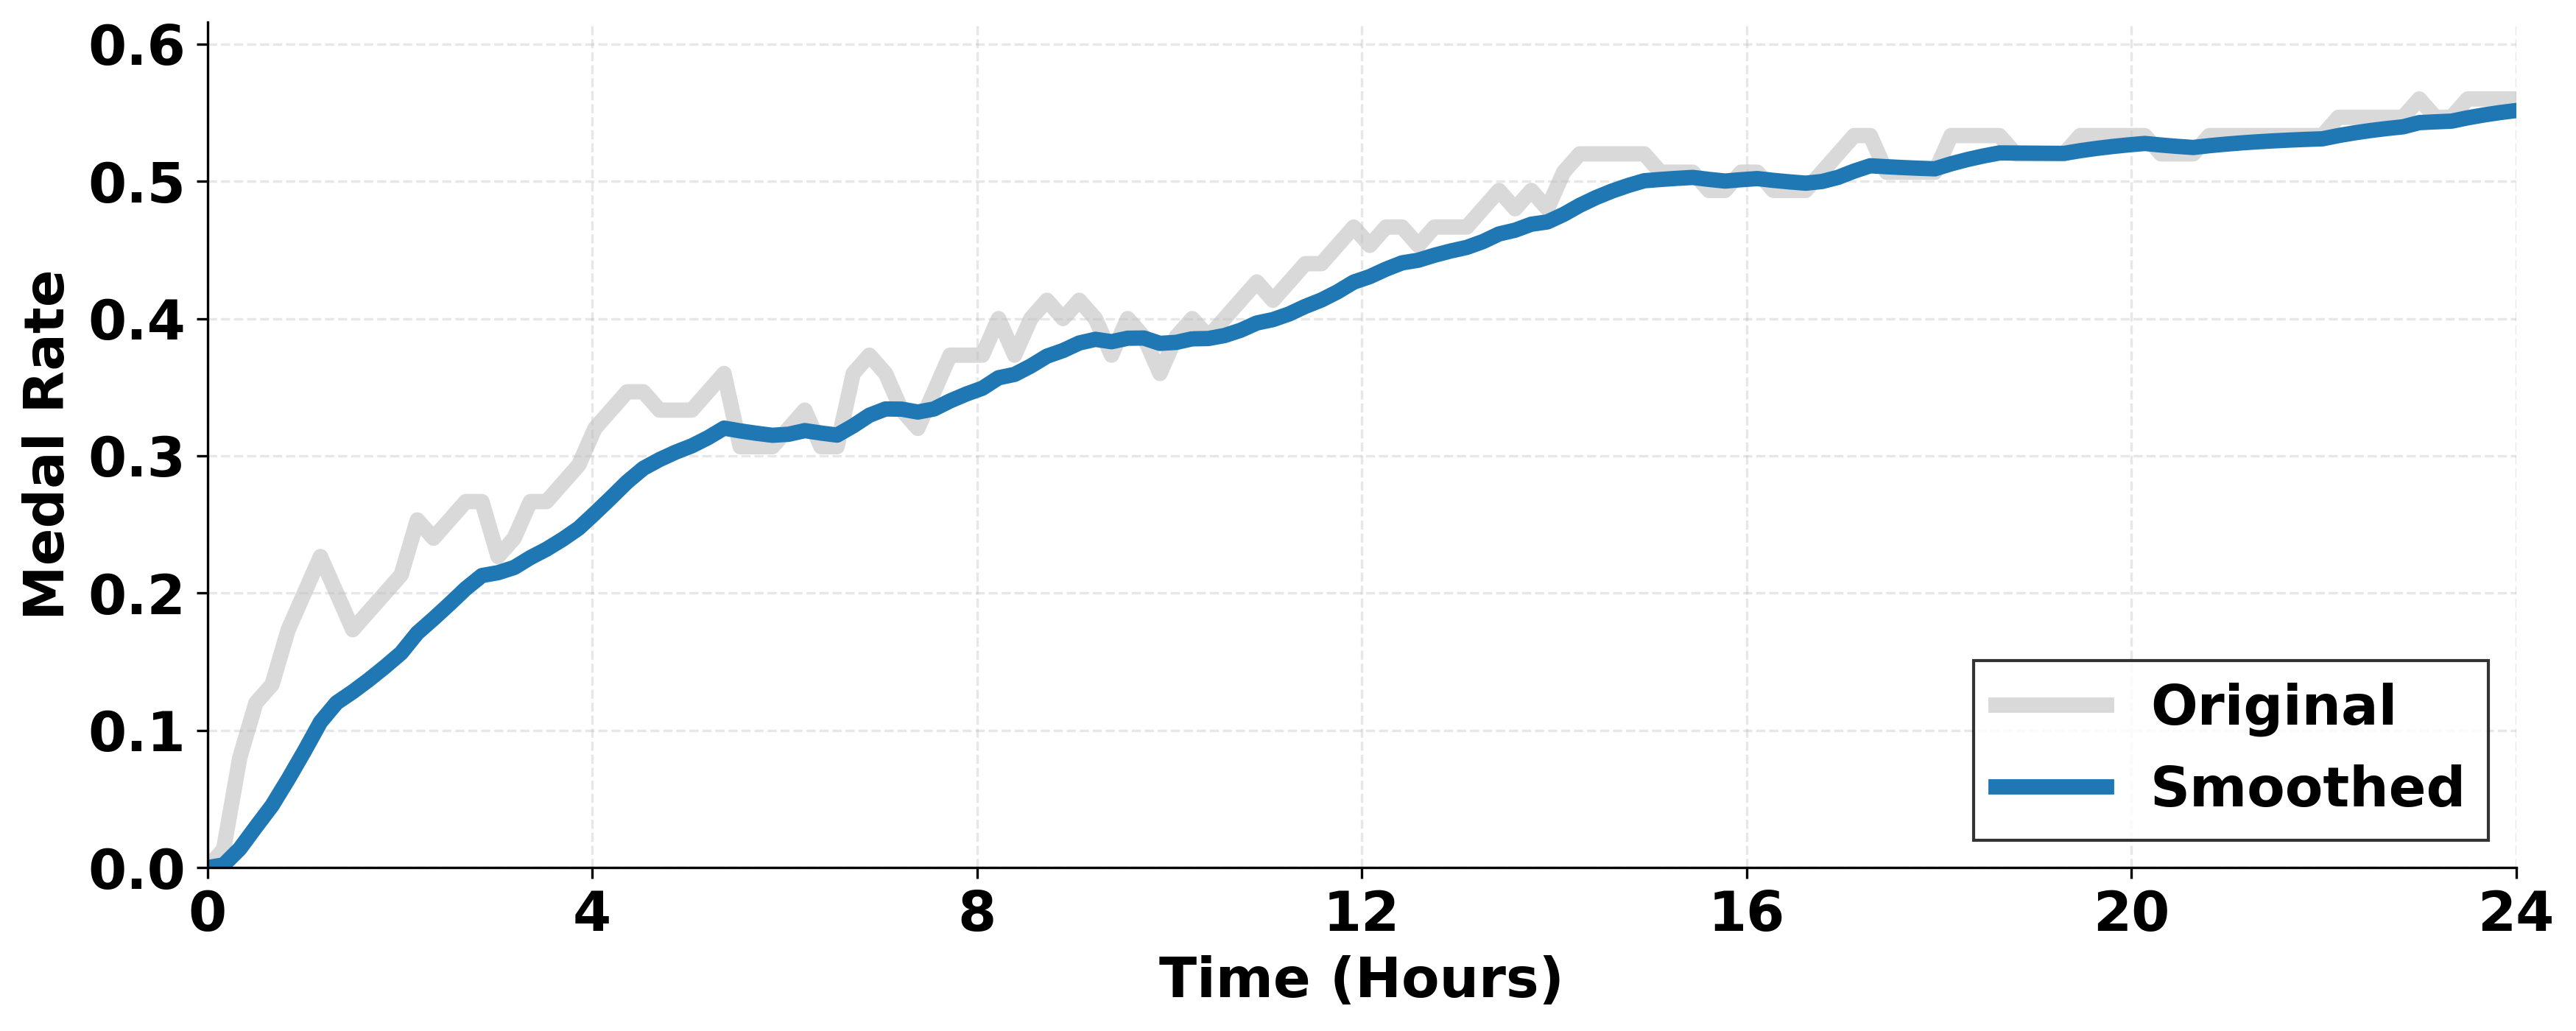
\includegraphics[width=1\textwidth]{figures/mlebench_time_medal.png}
    \caption{Evolving performance improvement of EvoMaster on MLE-Bench over time.}
    \label{fig:mlebench_time_medal}
\end{figure}

\subsection{Contributions}

Our main contributions are:

\begin{enumerate}[leftmargin=*, nosep]
    \item \textbf{The EvoMaster foundational agent framework.} We propose EvoMaster, a foundational evolving agent framework for agentic science at scale that enables new domain agents to be built in approximately 100 lines of code. EvoMaster also supports being invoked as a skill for other agents.
    \item \textbf{The SciMaster agent ecosystem.} We build 6+ autonomous research agents across diverse scientific domains on top of EvoMaster, facilitating a shared foundational harness enables rapid scaling to new disciplines.
    \item \textbf{Comprehensive experimental validation.} On four authoritative benchmarks, EvoMaster consistently outperforms OpenClaw with relative improvements of 159\% to 316\%, confirming the effectiveness of an evolution-driven foundational framework for scientific agents.
\end{enumerate}

%=====================================================================
\section{Related Work}
\label{sec:related}
%=====================================================================

\subsection{Agent Frameworks}

The landscape of LLM agent development is currently dominated by two paradigms. General-purpose orchestration frameworks like LangChain~\citep{langchain2025} and LangGraph~\citep{langgraph2025} provide foundational graph execution, while ecosystem-specific tools such as the OpenAI~\citep{openai2025agents}, Claude~\citep{anthropic2025claude}, and Google ADK~\citep{google2025adk} SDKs prioritize production-grade integration with proprietary models. In the open-source community, specialized frameworks have achieved significant traction: OpenHands~\citep{wang2025openhands, wang2025openhands_sdk} optimizes software engineering via event-sourced state models, while OpenClaw~\citep{steinberger2025openclaw} leverages an extensive skill ecosystem for rapid adoption.

Despite their success, these frameworks are primarily tailored for software development or general automation. They lack systematic support for the unique demands of scientific research, such as long-running experiment management and domain-specific knowledge injection. \textbf{EvoMaster} addresses this gap as a \textit{foundational} and \textit{evolving} framework, providing a cross-disciplinary base that aligns with the iterative nature of scientific discovery and scales seamlessly across diverse research domains.

\subsection{Scientific Agents}

The evolution of scientific agents has transitioned from early automated systems like the Robot Scientist~\citep{king2009automation} to modern LLM-driven architectures. Domain-specific agents have shown remarkable results: ChemCrow~\citep{bran2024augmenting} and Coscientist~\citep{boiko2023autonomous} automate chemical synthesis and robotic control, while specialized systems like Virtual Lab~\citep{swansonvirtuallab} and PaperQA2~\citep{zheng2025paperqa} excel in nanobody design and literature synthesis. Recent breakthroughs such as Google’s AI Co-Scientist~\citep{gottweis2025coscientist} and AI Scientist v2~\citep{aiscientistv2} further demonstrate the potential for agents to surpass human-level performance in hypothesis generation and peer-reviewed paper production. In machine learning, MLAgentBench~\citep{huang2023mlagentbench} and our previous work ML-Master~\citep{sjtu2025mlmaster} pioneered autonomous experimentation, supported by benchmarks like ScienceAgentBench~\citep{chen2025scienceagentbench}.

However, most existing scientific agents are implemented as end-to-end systems, leading to redundant engineering in tool and harness management. \textbf{EvoMaster} distinguishes itself by serving as the underlying framework layer. By abstracting essential scientific workflows, it enables developers to build self-evolving agents that iterate through experiments, effectively bridging the gap between bespoke scientific tools and a universal, scalable research harness.


%=====================================================================
\section{Design Principles}
\label{sec:principles}
%=====================================================================

EvoMaster's architecture is driven by the practical demands of scientific discovery. To realize our two core tenets—serving as a \textbf{foundational} framework and enabling continuous \textbf{evolution}—we establish four design principles. \textit{Modular Composability} and \textit{Experiment-Ready Harness} provide a foundational, scalable platform across disciplines, while \textit{Iterative Self-evolution} and \textit{Multi-Agent Collaborative Evolution} drive the evolutionary dynamics inherent to the scientific method.

\subsection{Modular Composability}

Monolithic agent systems couple decision logic with domain-specific tools, resisting cross-domain adaptation. EvoMaster achieves foundational flexibility by decoupling the architecture into orthogonal components across three layers: \textit{Playground}, \textit{Experiment} and \textit{Agent}.

Through unified registries and adherence to industry standards like the Model Context Protocol (MCP)~\citep{mcp2025} and Skill~\citep{anthropic2025skills}, developers can seamlessly swap models, environments, or toolsets. This composability drastically reduces the barrier to entry, enabling the deployment of new domain-specific scientific agents in approximately 100 lines of code.

\subsection{Experiment-Ready Harness}

Scientific research demands rigorous parameter control and absolute reproducibility. EvoMaster treats experimentation as a first-class primitive through two core mechanisms. First, a \textit{configuration-driven design} utilizes YAML-based manifests to manage agent parameters, prompts, and tool configurations dynamically, ensuring parameter agility without altering source code. 

Second, \textit{comprehensive observability} is achieved via a robust trajectory recording system. This system meticulously logs every conversational turn, tool invocation, and token statistic into thread-safe structured JSON. Just as researchers maintain strict laboratory notebooks, this guarantees that multi-turn agent experiments remain fully auditable and reproducible.

\subsection{Iterative Self-Evolving}

Unlike traditional agents that execute tasks linearly, scientific discovery relies on iterative cycles of hypothesis, observation, and revision. EvoMaster embeds this self-evolving loop directly into the Agent Engine. 

Operating within a multi-turn reactive architecture, agents continuously execute tools, observe experimental outcomes, and explicitly self-critique before determining the next action. To sustain these long-horizon evolutionary loops, EvoMaster integrates an intelligent Context Manager featuring dynamic LLM-based summarization and context compression, preventing context degradation over hundreds of experimental turns.

\subsection{Multi-Agent Collaborative Evolution}

Complex scientific problems frequently exceed the capacity of a single agent. EvoMaster’s Playground orchestration layer simulates real-world interdisciplinary collaboration by supporting dynamic multi-agent topologies. 

By declaratively defining Agent Slots, developers can orchestrate specialized agent teams. For example, when a critic agent identifies flaws in a solver's reasoning, the resulting revision represents a collaborative co-evolution, elevating the system's collective problem-solving capability beyond individual limits.

%=====================================================================
\section{Architecture}
\label{sec:architecture}
%=====================================================================

EvoMaster's architecture translates our design principles into a concrete system built specifically for the demands of scientific discovery. To break down domain silos and facilitate rapid \textbf{scale-up}, the framework is decoupled across execution and capability layers, ensuring a \textbf{foundational} harness that is seamlessly reusable across disciplines. To mirror the scientific method, the core engine and orchestration layers are fundamentally designed around \textbf{continuous evolution}, enabling agents to iteratively refine hypotheses, learn from feedback, and collaborate. As illustrated in Figure~\ref{fig:framework}, this architecture empowers developers to deploy self-evolving scientific agents with minimal overhead, maintaining strict correspondence between identified research bottlenecks and our structural solutions.

\begin{figure}[t]
    \centering
    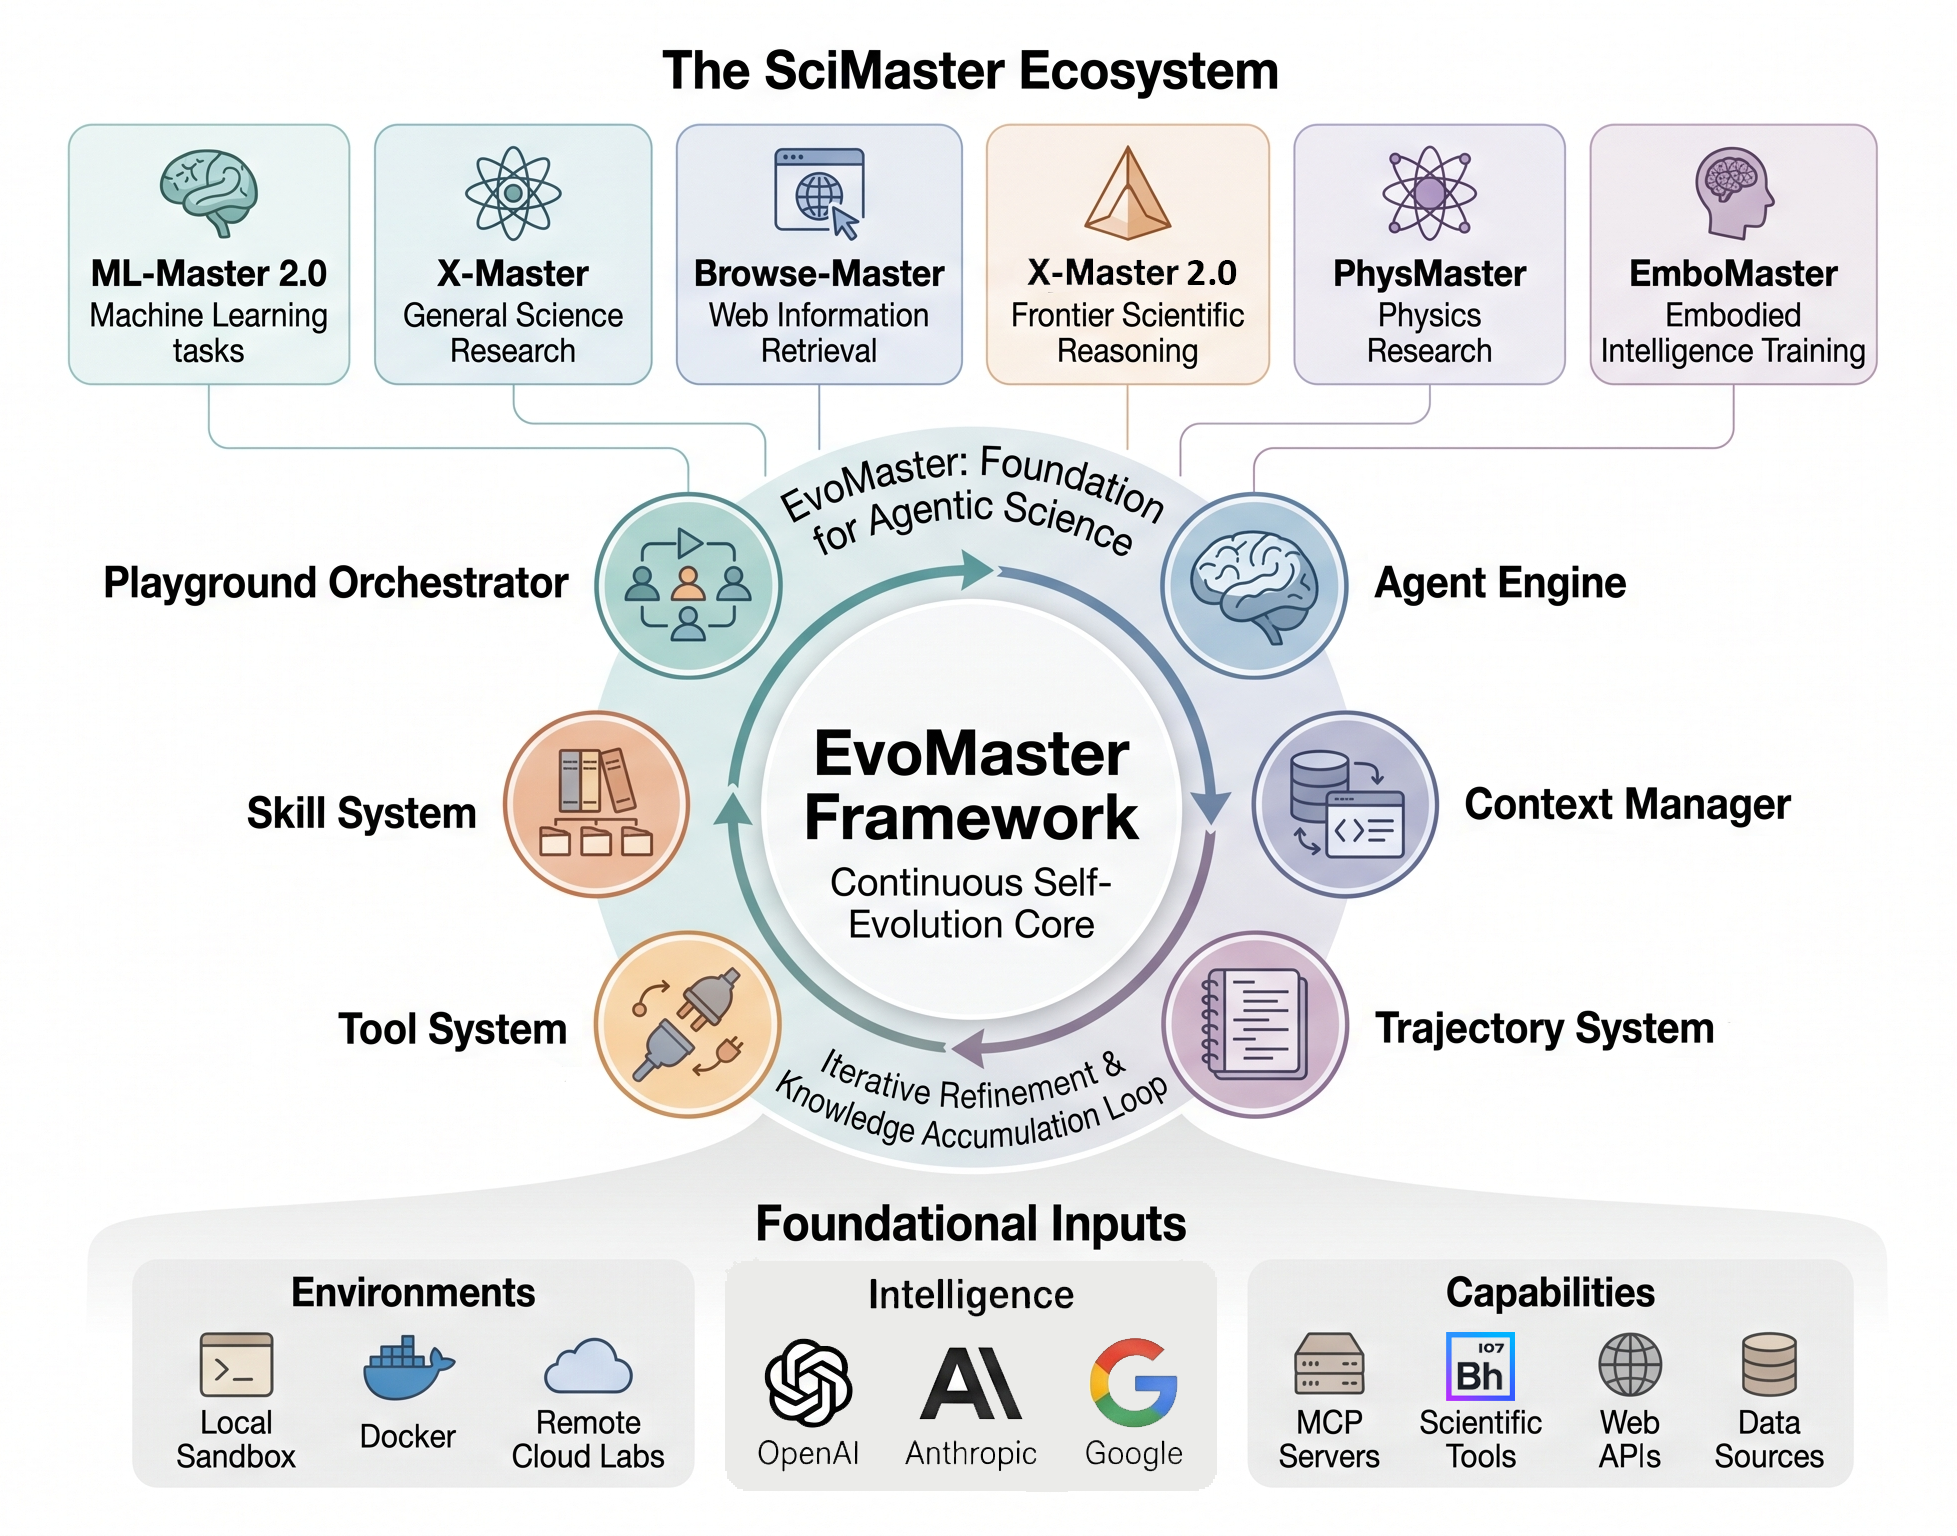
\includegraphics[width=\textwidth]{figures/framework_final_final.png}
    \caption{Overall architecture of EvoMaster.}
    \label{fig:framework}
\end{figure}

\subsection{Execution Architecture: Scaling Through Decoupling}

To overcome fragmented, siloed development and enable horizontal scaling across domains, EvoMaster structurally realizes \emph{Modular Composability} by separating execution into three orthogonal layers:
\begin{itemize}[leftmargin=*, nosep]
    \item \textbf{Playground (Orchestration):} Coordinates multi-agent collaboration patterns and domain-specific scientific workflows.
    \item \textbf{Exp (Experiment Execution):} Manages the single-experiment lifecycle, including task instantiation and trajectory recording.
    \item \textbf{Agent (Intelligence):} Drives the iterative reasoning and tool-use loop.
\end{itemize}
This separation guarantees that foundational improvements such as enhanced context management in the Agent Engine and benefit all scientific domains simultaneously. Expanding to a new discipline simply requires defining a new Playground, leaving the underlying execution and reasoning logic untouched.

\subsection{Agent Engine: The Evolution Core}

Traditional agents execute tasks in a single pass, contradicting the trial-and-error nature of scientific discovery. Addressing this, the Agent Engine serves as the realization of \emph{Iterative Self-Evolving}. Driven by the \texttt{BaseAgent} abstraction, it executes a multi-turn reactive loop: \textit{reason $\rightarrow$ invoke tools $\rightarrow$ observe $\rightarrow$ self-critique}. 

Since scientific tasks often span hundreds of interaction turns, maintaining this evolutionary loop requires robust memory. The engine integrates an intelligent \texttt{ContextManager} that prevents context degradation using dynamic LLM-based summarization and sliding windows. This ensures agents can accumulate insights and refine strategies over long experimental horizons without exceeding context limits.

\subsection{Capability Layer: Universal Tools and Skills}

This layer is the architectural realization of \emph{Modular Composability} at the capability level, providing the extensible mechanisms through which agents interact with scientific tools, domain knowledge, and language models. It is this layer that makes EvoMaster foundational: by providing a universal capability interface, it ensures that domain-specific extensions developed for one scientific discipline are immediately available to all others.

\begin{itemize}[leftmargin=*, nosep]
    \item \textbf{Tool System:} Utilizing an Action-Execution-Observation pattern, this system natively integrates with the Model Context Protocol (MCP)~\citep{mcp2025}. External MCP-compatible scientific tools are instantly converted into standard EvoMaster tools, unlocking a massive, cross-disciplinary tool ecosystem.
    \item \textbf{Skill System:} Adopting emerging skill specifications~\citep{anthropic2025skills}, domain knowledge is injected hierarchically. Metadata remains in-context for agent awareness, while detailed executable instructions are loaded on-demand to optimize context efficiency.
    \item \textbf{LLM Abstraction:} A unified interface standardizes responses across 100+ models~\citep{litellm2024}, allowing researchers to seamlessly swap backend models for controlled experimentation without altering agent logic.
\end{itemize}

\subsection{Playground Orchestrator: Collaborative Evolution}

Complex scientific problems frequently exceed single-agent capacities. The Playground orchestrator addresses this by materializing \emph{Multi-Agent Collaborative Evolution}. Developers use the \texttt{AgentSlots} mechanism to declaratively assign specialized roles (e.g., \textit{solver, critic, rewriter}), each maintaining independent LLM and tool configurations. 

The orchestrator natively supports diverse collaboration patterns, including sequential handoffs, parallel exploration, and iterative peer-review cycles. Through the \texttt{@register\_playground} decorator, custom workflow logic is automatically discovered at runtime. By reusing the shared foundational harness, developing a complex multi-agent scientific team is reduced to approximately 100 lines of orchestration code.

\subsection{Experiment Harness: Rigor and Reproducibility}

Scientific research demands absolute parameter control and auditability. Embodying the \emph{Experiment-Ready Harness} principle, EvoMaster treats every agent execution as a rigorous, reproducible experiment. 

All agent behaviors, prompts, and environment parameters are managed dynamically via YAML-based \textbf{Configuration Manifests}, allowing researchers to share complete experimental setups just like laboratory protocols. Furthermore, the \textbf{Trajectory System} acts as an automated lab notebook, meticulously logging every multi-turn dialogue, tool invocation, and token statistic into thread-safe, structured JSON. This guarantees that long-horizon evolutionary loops remain fully auditable and reproducible.

%=====================================================================
\section{The SciMaster Agent Ecosystem}
\label{sec:scimaster}
%=====================================================================

Built on the EvoMaster framework, we have constructed a growing ecosystem of autonomous research agents, collectively known as the SciMaster series (Table~\ref{tab:scimaster}). The ecosystem has already scaled to cover several distinct scientific domains, from autonomous machine learning to embodied intelligence training, and we are actively expanding to additional disciplines. 

\begin{table}[h]
\centering
\caption{The SciMaster agent ecosystem built on EvoMaster.}
\label{tab:scimaster}
\begin{tabular}{lll}
\toprule
\textbf{Agent} & \textbf{Domain} & \textbf{Code Status} \\
\midrule
ML-Master 2.0~\citep{sjtu2026mlmaster2} & Autonomous Machine Learning & Open-sourced \\
ML-Master~\citep{sjtu2025mlmaster} & Autonomous Machine Learning & Open-sourced \\
X-Master~\citep{sjtu2025xmaster} & General Scientific Research & Open-sourced \\
Browse-Master~\citep{sjtu2025browsemaster} & Web Information Retrieval & Open-sourced \\
X-Master 2.0 & Frontier Scientific Reasoning & Coming soon \\
PhysMaster~\citep{sjtu2025physmaster} & Physics Research \& Reasoning & Coming soon \\
EmboMaster~\citep{sjtu2026embomaster} & Embodied Intelligence Training & Coming soon \\
\bottomrule
\end{tabular}
\end{table}

The rapid expansion of the SciMaster ecosystem underscores the profound advantages of building domain-specific agents atop the EvoMaster foundational harness. Rather than developing isolated systems from scratch, incubating agents within this framework yields three critical architectural benefits, which reduces the time required for developers to build specialized agents from several days to mere hours:

\begin{itemize}[leftmargin=*, nosep]
    \item \textbf{Drastic Reduction in Engineering Overhead.} By inheriting EvoMaster's unified Agent Engine, context management, and Playground orchestrator, developers avoid redundant harness coding. 
    \item \textbf{Shared Evolutionary Upgrades.} Since the execution logic is completely decoupled from domain knowledge, core algorithmic enhancements immediately benefit the entire ecosystem. 
    \item \textbf{Cross-Domain Tool Interoperability.} Leveraging the standardized Capability Layer, tools developed for one discipline become universally accessible. A specialized skill or script can be seamlessly invoked to another agent, fostering genuine interdisciplinary cross-pollination.
\end{itemize}

By centralizing the complex machinery of continuous evolution and orchestration, EvoMaster frees researchers to focus exclusively on domain-specific scientific logic, proving itself as the optimal and highly scalable substrate for the next generation of Agentic Science.


%=====================================================================
\section{Experiments}
\label{sec:experiments}
%=====================================================================

\subsection{Benchmarks}

We evaluate EvoMaster on four authoritative benchmarks spanning diverse capability dimensions: \textbf{HLE}~\citep{hle2025} for cross-disciplinary expert knowledge, \textbf{MLE-Bench (Lite)}~\citep{chan2024mlebench} for ML engineering, \textbf{BrowseComp}~\citep{wei2025browsecomp} for deep web retrieval, and \textbf{FrontierScience}~\citep{openai2026frontierscience} for frontier scientific reasoning across physics, chemistry, and biology. Detailed benchmark descriptions are provided in Appendix~\ref{sec:benchmark_details}.

\subsection{Experimental Setup}

We compare EvoMaster against \textbf{OpenClaw}~\citep{steinberger2025openclaw}, one of the fastest-growing open-source AI agent projects in 2025--2026. OpenClaw supports 100+ built-in skills and multi-platform integration, and serves as a representative example of recent general-purpose AI agent systems.

In our experiments, EvoMaster uses its standard configuration to run SciMaster series agents tailored to each benchmark. Specifically:
\begin{itemize}[leftmargin=*, nosep]
    \item \textbf{HLE}: X-Master~\citep{sjtu2025xmaster}, configured for cross-disciplinary scientific reasoning.
    \item \textbf{MLE-Bench (Lite)}: ML-Master~2.0~\citep{sjtu2026mlmaster2}, with its multi-phase iterative optimization pipeline featuring research-driven parallel improvement and hierarchical cognitive caching architecture.
    \item \textbf{BrowseComp}: Browse-Master~\citep{sjtu2025browsemaster}, using a Planner-Executor iterative loop for progressive information retrieval.
    \item \textbf{FrontierScience}: X-Master 2.0, a single-agent solver enhanced with academic retrieval tools for frontier scientific reasoning.
\end{itemize}
To ensure a fair comparison, all experiments were conducted on an NVIDIA RTX 4090 GPU server. Both approaches utilize GPT-5.4 as the backend model and are equipped with identical tools and skills. Additionally, we imposed a strict 24-hour runtime limit for the MLE-Bench evaluation.

\subsection{Results and Analysis}

Table~\ref{tab:results} presents the comparison between EvoMaster and OpenClaw across four benchmarks.

\begin{table}[t]
\centering
\caption{Benchmark comparison between EvoMaster and OpenClaw. EvoMaster consistently outperforms OpenClaw across all four benchmarks with relative improvements ranging from 159\% to 316\%.}
\label{tab:results}
\begin{tabular}{lcc>{\columncolor{lightgreen}}c}
\toprule
\textbf{Benchmark} & \textbf{OpenClaw} & \textbf{EvoMaster} & \textbf{Rel.\ Improvement} \\
\midrule
HLE & 13.6 & \textbf{41.1} & +202\% \\
MLE-Bench (Lite) & 18.2 & \textbf{75.8} & +316\% \\
BrowseComp & 28.3 & \textbf{73.3} & +159\% \\
FrontierScience & 18.3 & \textbf{53.3} & +191\% \\
\bottomrule
\end{tabular}
\end{table}



\textbf{MLE-Bench (+316\%).} EvoMaster achieves 75.8\% compared to OpenClaw's 18.2\%, the largest margin among all benchmarks. EvoMaster earns medals on approximately 17 of 22 Kaggle competitions, while OpenClaw manages only 4 despite submitting on 18. The gap stems from EvoMaster's multi-phase iterative workflow: knowledge prefetch retrieves past insights, a drafting stage generates an initial solution, then up to 20 rounds of research-driven parallel improvement progressively refine it. A hierarchical cognitive caching mechanism (spanning prefetch, round-level knowledge promotion, and run-level wisdom promotion) accumulates reusable experience across cycles, embodying the evolution philosophy at the framework's core.

\begin{table}[ht]
\centering
\small
\caption{\textbf{Evaluation Results on MLE-Bench(Lite).} We compare EvoMaster against OpenClaw, MLE-STAR-Pro-1.5~\citep{nam2025mle}, and R\&D-Agent~\citep{yang2025r} on MLE-Bench Lite. The best results in each metric are highlighted in \textbf{bold}. EvoMaster and OpenClaw use GPT-5.4 as the backend model and have a maximum runtime of 24 hours. We use the results of MLE-STAR-Pro-1.5 and R\&D-Agent reported by official MLE-Bench.}
\label{tab:mlebench_comparison}

\begin{tabular}{@{}l c c c c >{\columncolor{lightgreen}[0pt][0pt]}c@{}}
\toprule
\textbf{Metric} & \textbf{OpenClaw (Baseline)} & \textbf{MLE-STAR} & \textbf{R\&D-Agent} & \textbf{EvoMaster (Ours)} & \textbf{$\Delta$ (Gain)} \\ 
\midrule
Valid & 81.82 & \textbf{100.00} & 77.27 & \textbf{100.00} & +18.18 \\
Above Median      & 31.82 & 75.76 & 74.24 & \textbf{84.85}  & +53.03 \\ 
Bronze            & 4.55  & \textbf{16.67} & 12.12 & 13.64  & +9.09 \\
Silver            & 13.64 & 16.67 & 22.73 & \textbf{31.82}  & +18.18 \\
Gold              & 0.00  & \textbf{34.85} & 33.33 & 30.30  & +30.30 \\
\midrule
\cellcolor[gray]{0.9} Any Medal
& \cellcolor[gray]{0.9} 18.18
& \cellcolor[gray]{0.9} 68.18
& \cellcolor[gray]{0.9} 68.18
& \cellcolor[gray]{0.9} \textbf{75.76}
& \textbf{+57.58} \\
\bottomrule
\end{tabular}
\end{table}



\textbf{BrowseComp (+159\%).} EvoMaster achieves 73.3\% versus OpenClaw's 28.3\% on the BrowseComp benchmark. Through a Planner-Executor iterative loop (up to 10 rounds), the planner formulates targeted search plans based on accumulated findings, while the executor retrieves information via web search, URL fetching, and PDF extraction. This iterative deepening allows progressive query refinement and cross-source validation, whereas OpenClaw settles for the first plausible answer. The impact of this pipeline is evident across all question categories. EvoMaster consistently outperforms OpenClaw, with the most striking gain in Map + Search tasks (100.0\% vs 25.0\%, +75.0\%). This suggests that the iterative planning process effectively resolves the geographical reasoning bottlenecks inherent in complex retrieval. Furthermore, significant improvements in Niche Knowledge (+52.9\%) and Multi-step Reasoning (+43.8\%) highlight the framework's versatility, proving that structured agentic coordination can robustly bridge the gap between base model capability and expert-level information retrieval requirements.


\begin{table}[ht]
\centering
\small
\caption{\textbf{Evaluation Results on BrowseComp.} We compare the accuracy (\%) of EvoMaster against the OpenClaw across major subject categories. The best results in each category are highlighted in \textbf{bold}. Both methods use GPT-5.4 as the backend model.}
\label{tab:browse_comparison}
\begin{tabular}{@{}l c c >{\columncolor{lightgreen}[0pt][0pt]}c@{}}
\toprule
\textbf{Category} & \textbf{OpenClaw (Baseline)} & \textbf{EvoMaster (Ours)} & \textbf{$\Delta$ (Gain)} \\ 
\midrule
\quad Multi-step Reasoning & 18.75 & \textbf{65.63} & +46.88 \\
\quad Map + Search         & 25.00 & \textbf{75.00} & +50.00 \\
\quad Niche Knowledge      & 47.05 & \textbf{88.23} & +41.18 \\
\quad Complex Filtering    & 28.57 & \textbf{71.43} & +42.86 \\
\midrule
\cellcolor[gray]{0.9}\textbf{Overall}
& \cellcolor[gray]{0.9}\textbf{28.33}
& \cellcolor[gray]{0.9}\textbf{73.33}
& \textbf{+45.00} \\
\bottomrule
\end{tabular}
\end{table}


\textbf{FrontierScience (+191\%).} EvoMaster achieves 53.3\% compared to OpenClaw's 18.3\% on the Research track (open-ended subtasks). A single-agent architecture enhanced with academic retrieval tools (Google Scholar, Semantic Scholar API, PDF reader) enables iterative tool-driven reasoning: the agent retrieves relevant literature, reflects on findings, and refines its understanding before synthesizing answers grounded in verifiable sources.

\begin{table}[ht]
\centering
\small
\caption{\textbf{Evaluation Results on Frontier Science Research.} We compare the average normalized score (\%) of OpenClaw, GPT-5.4, Muse Spark, and EvoMaster across major scientific subject categories. The best results in each category are highlighted in \textbf{bold}. OpenClaw and EvoMaster use GPT-5.4 as the backend model. Due to constraints in time and computational resources, we currently report results from a single run.}
\label{tab:fs_research_comparison}
\begin{tabular}{@{}l c c c c >{\columncolor{lightgreen}[0pt][0pt]}c@{}}
\toprule
\textbf{Category} 
& \textbf{OpenClaw (Baseline)} 
& \textbf{GPT-5.4} 
& \textbf{Muse Spark} 
& \textbf{EvoMaster (Ours)} 
& \textbf{$\Delta$ (Gain)} \\
\midrule
\quad Physics   
& 15.00 
& - 
& - 
& \textbf{55.00} 
& +40.00 \\
\quad Chemistry 
& 20.00 
& - 
& - 
& \textbf{55.00} 
& +35.00 \\
\quad Biology   
& 20.00 
& - 
& - 
& \textbf{50.00} 
& +30.00 \\
\midrule
\cellcolor[gray]{0.9}\textbf{Overall}
& \cellcolor[gray]{0.9}18.33
& \cellcolor[gray]{0.9}33.00
& \cellcolor[gray]{0.9}38.30
& \cellcolor[gray]{0.9}\textbf{53.33}
& \textbf{+35.00} \\
\bottomrule
\end{tabular}
\end{table}



\textbf{HLE (+202\%).} EvoMaster achieves 41.1\% accuracy vs. 13.6\% for OpenClaw, driven by its four-phase parallel pipeline (Solve, Critique, Rewrite, Select), which enables structured multi-agent refinement. Solver agents generate candidates, critics identify errors, and rewriters iteratively improve outputs before selection.
This process is especially effective on hard HLE instances where initial solutions are weak. EvoMaster outperforms OpenClaw across all domains, with the largest gain in Mathematics (48.16\%, +33.10\%), followed by Computer Science (+24.55\%) and Humanities (+30.05\%), indicating strong cross-domain generalization.
Overall, structured agent coordination significantly enhances performance over the base model, particularly for multi-step reasoning tasks.


\begin{table}[ht]
\centering
\small
\caption{\textbf{Evaluation Results on HLE (Humanity's Last Exam).} We compare the accuracy (\%) of EvoMaster against OpenClaw, GPT-5.4 xhigh, and Muse Spark across major subject categories. The best results in each category are highlighted in \textbf{bold}. Both methods use GPT-5.4 as the backend model.}
\label{tab:hle_comparison}

\setlength{\tabcolsep}{4pt}
\renewcommand{\arraystretch}{1.08}

\begin{tabularx}{\linewidth}{@{}>{\raggedright\arraybackslash}X c c c c >{\columncolor{lightgreen}[0pt][0pt]}c@{}}
\toprule
\textbf{Category} & \textbf{OpenClaw} & \textbf{GPT-5.4} & \textbf{Muse} & \textbf{EvoMaster} & \textbf{$\Delta$} \\
& \textbf{(Baseline)} & \textbf{(xhigh)} & \textbf{Spark} & \textbf{(Ours)} & \textbf{(Gain)} \\
\midrule
\textit{STEM} & & & & & \\
\quad Biology / Medicine        & 14.86 & - & - & \textbf{29.28} & +14.42 \\
\quad Chemistry                 & 11.88 & - & - & \textbf{29.70} & +17.82 \\
\quad Computer Science / AI     & 12.50 & - & - & \textbf{37.05} & +24.55 \\
\quad Engineering               & 7.81  & - & - & \textbf{21.88} & +14.07 \\
\quad Math                      & 15.06 & - & - & \textbf{48.16} & +33.10 \\
\quad Physics                   & 13.86 & - & - & \textbf{31.68} & +17.82 \\
\midrule
\textit{Social Science \& Humanities} & & & & & \\
\quad Humanities / Social Science & 13.99 & - & - & \textbf{44.04} & +30.05 \\
\midrule
\textit{Others} & & & & & \\
\quad Other Categories          & 7.95  & - & - & \textbf{43.18} & +35.23 \\
\midrule
\rowcolor[gray]{0.9}
\textbf{Overall}
& {13.62}
& {36.47}
& {40.92}
& \textbf{41.10}
& \textbf{+27.48} \\
\bottomrule
\end{tabularx}
\end{table}




In conclusion, EvoMaster substantially outperforms OpenClaw across all four benchmarks, with relative improvements ranging from 159\% (BrowseComp) to 316\% (MLE-Bench Lite). This consistent advantage across fundamentally different task types---closed-book knowledge, ML engineering, web retrieval, and scientific reasoning---demonstrates that a foundational agent framework with evolving capabilities provides systematic benefits over general-purpose platforms.

%=====================================================================
\section{Conclusion}
\label{sec:conclusion}
%=====================================================================

In this paper, we introduced \textbf{EvoMaster}, a foundational and evolving agent framework designed to catalyze Agentic Science at Scale. Addressing the limitations of siloed and static agent architectures, EvoMaster is built upon the dual pillars of foundational modularity and continuous self-evolution. By deeply integrating iterative refinement loops, experiment-ready harness, and multi-agent collaborative workflows, EvoMaster mirrors the authentic scientific method---enabling agents to autonomously hypothesize, experiment, self-critique, and continuously evolve from trial and error.

Our comprehensive evaluation across four authoritative benchmarks (HLE, MLE-Bench Lite, BrowseComp, and FrontierScience) demonstrates that EvoMaster consistently and substantially outperforms the general-purpose framework OpenClaw, achieving relative performance improvements ranging from 159\% to 316\%. Furthermore, the successful incubation of the \textbf{SciMaster} ecosystem validates EvoMaster's cross-disciplinary scalability. By standardizing the foundational abstractions, the framework empowers researchers to rapidly deploy self-improving scientific agents across diverse domains with minimal engineering overhead.

Looking ahead, we envision EvoMaster serving as the foundationa substrate for autonomous scientific discovery. As we actively expand the framework to encompass broader disciplines---such as biochemistry, materials science, and complex physical systems---our ultimate goal is to shift the bottleneck of scientific progress from human bandwidth to scalable, self-evolving artificial intelligence.

\subsection*{Limitations}

While EvoMaster represents a substantial step toward scalable agentic science, we acknowledge the following limitation in its current scope:
\begin{itemize}[leftmargin=*, nosep]
    \item \textbf{Integration with physical environments.} At present, EvoMaster is primarily optimized for \emph{in silico} and computational research workflows. It lacks native support for executing tasks that require direct manipulation of physical experimental apparatuses, such as automated cloud labs or robotic synthesis hardware. Expanding the \texttt{Session} abstraction to bridge this gap and interface seamlessly with standard laboratory automation protocols remains a vital avenue for future research.
\end{itemize}


\newpage

\appendix

\section{Benchmark Descriptions}
\label{sec:benchmark_details}

This appendix provides detailed descriptions of the four evaluation benchmarks used in our experiments.

\textbf{Humanity's Last Exam (HLE)}~\citep{hle2025}. HLE is one of the most challenging closed-book knowledge assessments ever constructed. It aggregates 2,500 questions across dozens of academic disciplines, with mathematics (41\%), biology and medicine (11\%), computer science (10\%), physics (9\%), humanities and social sciences (9\%), chemistry (7\%), and others, contributed by nearly 1,000 experts from over 500 institutions across 50 countries. Approximately 14\% of questions are multimodal (requiring image understanding), while 24\% are multiple-choice and the remainder are short-answer exact-match.

\textbf{MLE-Bench}~\citep{chan2024mlebench}. MLE-Bench curates 75 real machine learning engineering competitions from Kaggle spanning 15 diverse categories including NLP, computer vision, and signal processing. Agents must complete the full ML pipeline including data processing, feature engineering, model selection, training, and submission. The evaluation metric is the overall average any medal rate (achieving at least bronze medal performance on the competition leaderboard).

\textbf{BrowseComp}~\citep{wei2025browsecomp}. BrowseComp comprises 1,266 complex web information retrieval tasks. BrowseComp requires agents to persistently navigate tens or hundreds of web pages to locate entangled information: facts that cannot be found with a single query but demand creative, multi-step browsing strategies and cross-source validation. The benchmark is intentionally designed to test an agent's ability to adapt search strategies, synthesize information across sources, and persist through challenging retrieval scenarios.

\textbf{FrontierScience}~\citep{openai2026frontierscience}. FrontierScience evaluates AI agents on frontier scientific reasoning across three natural science disciplines: physics, chemistry, and biology. It comprises two complementary tracks: the Olympiad track contains 100 problems designed by international competition gold medalists (at IPhO, IChO, and IBO level), evaluated via short-answer exact-match; the Research track contains 60 original research subtasks designed by PhD scientists, graded on a 10-point rubric for scientific rigor and methodology. FrontierScience targets natural science reasoning, a domain particularly relevant to Agentic Science.

\newpage
\bibliography{main}

\end{document}
